\documentclass[a4paper]{oblivoir}
\usepackage{amsmath,amssymb,kotex,mdframed,paralist,graphicx,caption}
\usepackage{fapapersize}
%\usefapapersize{210mm,297mm,10mm,*,10mm,*}

\usepackage{multicol}
\setlength{\columnsep}{30pt}
\setlength{\columnseprule}{1pt}

\usepackage{tabto,pifont}
%\TabPositions{0.1\textwidth,0.2\textwidth,0.3\textwidth,0.4\textwidth}
%\renewcommand\fontsize{small}\selectfont 


%%% 객관식 선지
\newcommand\one{\ding{172}}
\newcommand\two{\ding{173}}
\newcommand\three{\ding{174}}
\newcommand\four{\ding{175}}
\newcommand\five{\ding{176}}
\usepackage{tabto,pifont}
%\TabPositions{0.2\textwidth,0.4\textwidth,0.6\textwidth,0.8\textwidth}

\newcommand\taba[5]{\par\noindent
\one\:{#1}
\tabto{0.2\textwidth}\two\:\:{#2}
\tabto{0.4\textwidth}\three\:\:{#3}
\tabto{0.6\textwidth}\four\:\:{#4}
\tabto{0.8\textwidth}\five\:\:{#5}}

\newcommand\tabb[5]{\par\noindent
\one\:{#1}
\tabto{0.33\textwidth}\two\:\:{#2}
\tabto{0.67\textwidth}\three\:\:{#3}\medskip\par\noindent
\four\:\:{#4}
\tabto{0.33\textwidth}\five\:\:{#5}}

\newcommand\tabc[5]{\par\noindent
\one\:{#1}
\tabto{0.5\textwidth}\two\:\:{#2}\medskip\par\noindent
\three\:\:{#3}
\tabto{0.5\textwidth}\four\:\:{#4}\medskip\par\noindent
\five\:\:{#5}}

\newcommand\tabd[5]{\par\noindent
\one\:{#1}\medskip\par\noindent
\two\:\:{#2}\medskip\par\noindent
\three\:\:{#3}\medskip\par\noindent
\four\:\:{#4}\medskip\par\noindent
\five\:\:{#5}}

\newcommand\vs[1]{\par\vspace{30pt}}

\usepackage{graphicx}

%\pagestyle{empty}

%%% Counters
\newcounter{num}

%%% Commands
\newcommand{\prob}[1]
{\bigskip\bigskip\noindent\refstepcounter{num}\textbf{문제 \arabic{num})} #1\par\noindent}

\newcommand\pb[1]{\ensuremath{\fbox{\phantom{#1}}}}

\newcommand\ba{\ensuremath{\:|\:}}

\newcommand\an[1]{\bigskip\par\noindent\textbf{문제 #1)}\par\noindent}

%%% Meta Commands
\let\oldsection\section
\renewcommand\section{\clearpage\oldsection}

\let\emph\textsf

\begin{document}
\title{태희 : 2019학년도 수능 관련}
\date{\today}
\author{}
\maketitle

\begin{multicols*}{2}
%
\prob{가형 14번}
\begin{center}
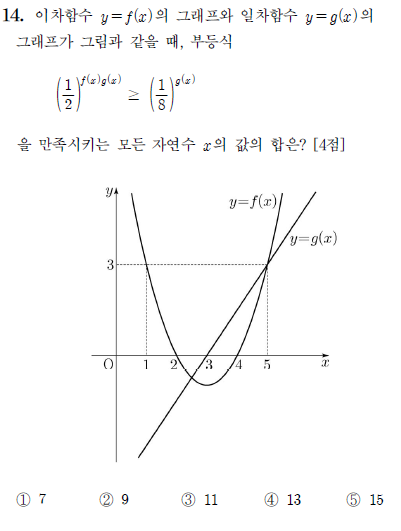
\includegraphics[width=\columnwidth]{+14}
\end{center}
\vfill\null\columnbreak
주어진 부등식을 간단히 하면
\begin{align*}
&\left(\frac12\right)^{f(x)g(x)}\ge\left(\frac12\right)^{3g(x)}\\
\iff& f(x)g(x)\le3g(x)\\
\iff& g(x)\big(f(x)-3\big)\le0\\
\iff& \Big[\big(g(x)\ge0\big)\wedge\big(f(x)\le3\big)\Big]\vee\Big[\big(g(x)\le0\big)\wedge\big(f(x)\ge3\big)\Big]\\
\iff& \Big[\big(x\ge3\big)\wedge\big(1\le x\le 5\big)\Big]\vee\Big[\pb{\(x\le3\)}\wedge\pb{\(x\le1\vee x\ge5\)}\Big]\\
\iff& \Big[1\le x\le 5\Big]\vee\Big[\pb{\(1\le x\le 5\)}\Big]
\end{align*}
\end{multicols*}

\newpage
\begin{multicols*}{2}
%
\prob{가형 17번(나형 19번)}
\begin{center}
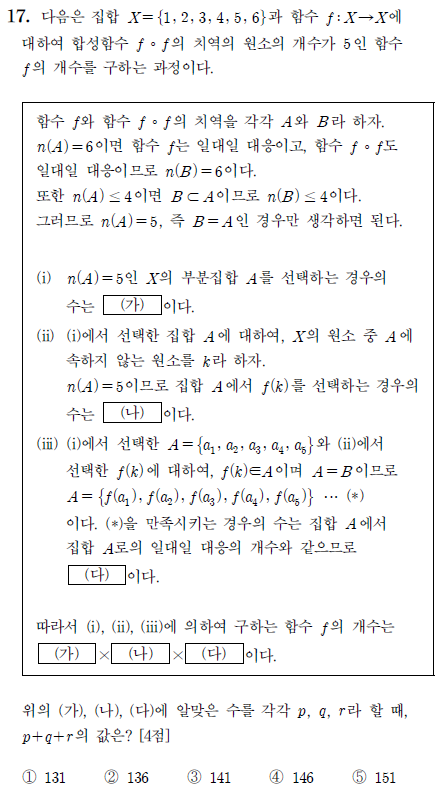
\includegraphics[width=\columnwidth]{+17}
\end{center}
\vfill\null

\begin{center}
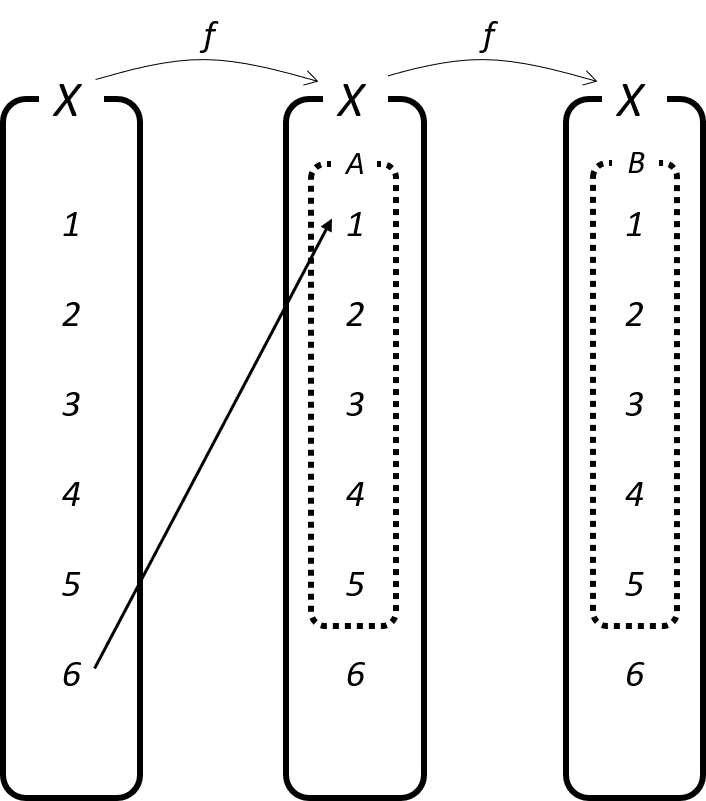
\includegraphics[width=.8\columnwidth]{+17_1}
\end{center}
\vfill\null\columnbreak
\noindent(가) :
\(X\)의 부분집합 중에서 원소의 개수가 5개인 것은
\begin{gather*}
\{1,2,3,4,5\},
\{1,2,3,4,6\},
\{1,2,3,5,6\},\\
\{1,2,4,5,6\},
\{1,3,4,5,6\},
\{2,3,4,5,6\}
\end{gather*}
의 6가지이다.
이것은 \(_6C_5\)를 계산하여 구할 수도 있다.

\bigskip\noindent(나) :
일반성을 잃지 않고\\ \(A=\{1,2,3,4,5\}\)라고 가정하자.\\
따라서 \(k=6\)이다.
이때, \(f(6)\)의 값으로 가능한 것은
\begin{align*}
&f(6)=1,\quad f(6)=2,\quad f(6)=3,\\
&f(6)=4,\quad f(6)=5
\end{align*}
의 5가지이다.
%\(f(6)=6\)이 될 수는 없다.
%\(6\)은 \(f\)의 치역(\(=A\))에 속하지 않기 때문이다.

\bigskip\noindent(다) :
일반성을 잃지 않고 \(f(6)=1\)이라고 가정하자.
이제 \(f(1)\), \(f(2)\), \(f(3)\), \(f(4)\), \(f(5)\)를 정하면 함수는\\ 완성된다.
이 값들은 1, 2, 3, 4, 5 중 하나이므로 결국
\(A=\{1,2,3,4,5\}\)에서 \(B(=A)\)로 가는 함수\\ \(g:A\to B\)를 생각하면 된다.

\medskip
만약 \(g\)가 일대일 대응이 아니면 \(g\)의 치역은 \(B\)의 진부분집합이다.
따라서 \(f\circ f\)의 치역도 \(B\)가 아니게 된다.
만약 \(g\)가 일대일 대응이면 \(f\circ f\)의 치역이 \(B\)가 된다. 따라서 주어진 조건을 모두 만족시킨다.

\medskip
\(A\)에서 \(B\)로 가는 일대일 대응\\ \(g\)의 개수는 \(_\square P_\square=\square!=\pb{120}\)가지이다.

%\(B\)는 \(f\circ f\)의 치역이므로
%\[B=\{f(f(x))\ba x=1,2,3,4,5,6\}\]
%이다.
%그런데 \(f(x)\)는 \(1,2,3,4,5\)의 값만 가질 수 있으므로
%\begin{align*}
%B
%&=\{f(t)\ba t=1,2,3,4,5\}\\
%&=\{f(1),f(2),f(3),f(4),f(5)\}
%\end{align*}
%따라서 \(A=\{1,2,3,4,5\}\)와 \(B=\{f(1),f(2),f(3),f(4),f(5)\}\) 사이의 일대일 대응을 만들면 그것으로부터 함수 \(f\)를 만들 수 있다.
%\(A\)와 \(B\) 사이의 일대일 대응의 개수는 \(_5P_5=5!=120\)가지이다.
\end{multicols*}
\newpage
\(g:A\to B\)가 일대일 대응이면 그로부터 \(f\circ f\)의 치역의 원소의 개수가 5인 함수 \(f\)를 만들 수 있다.
\begin{center}
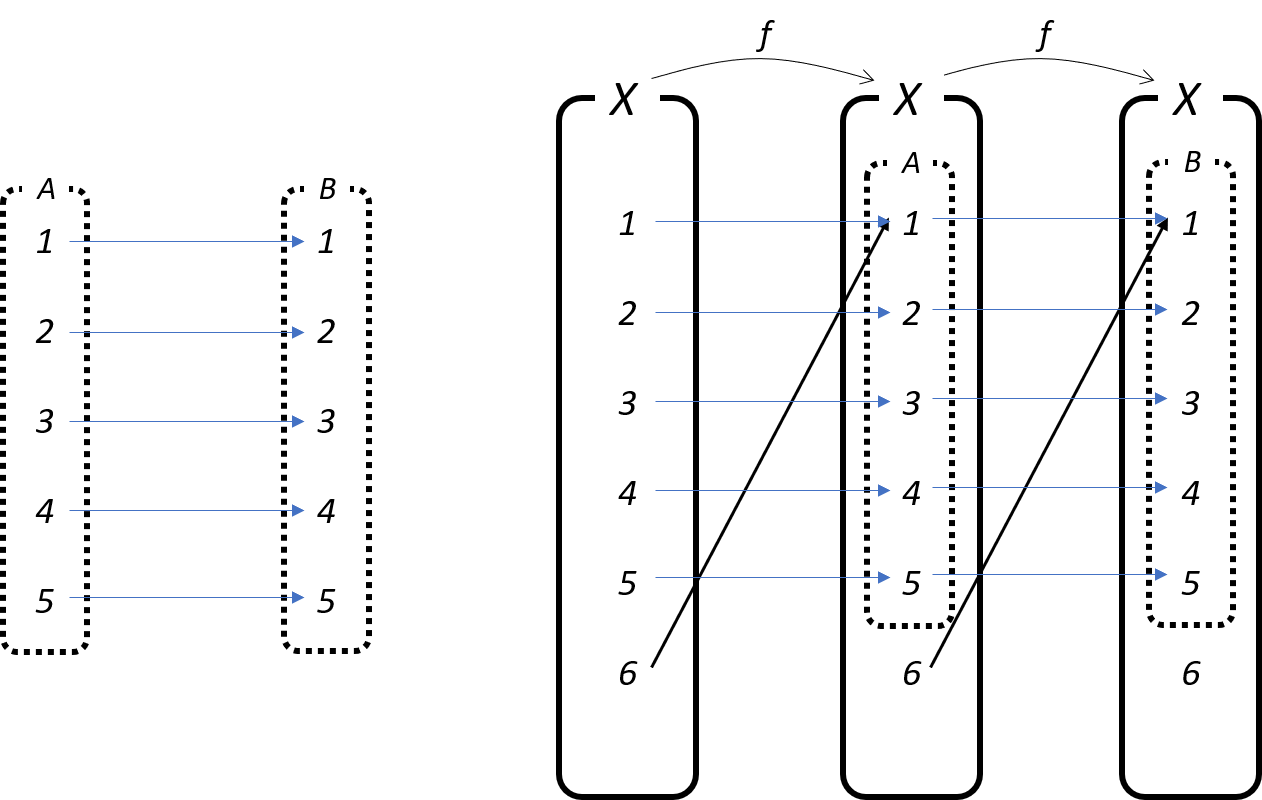
\includegraphics[width=.5\columnwidth]{+17_2}
\par
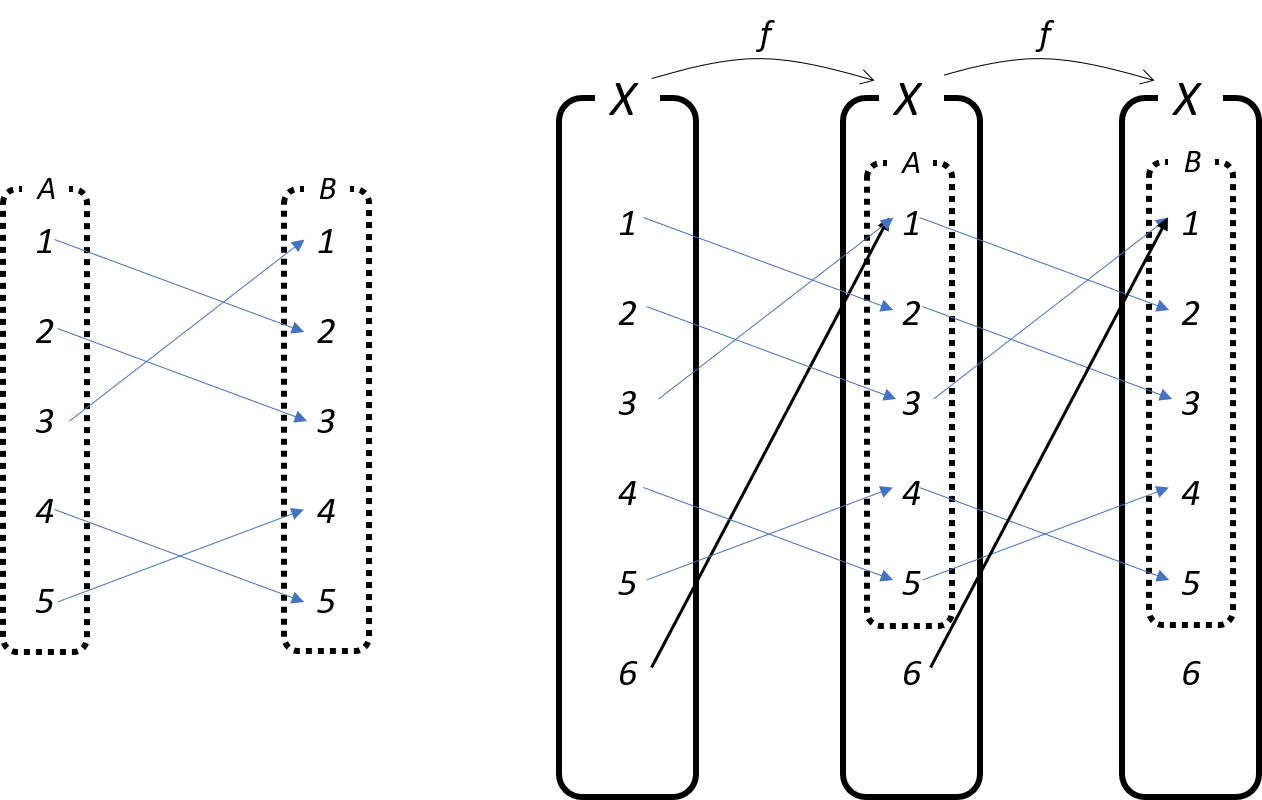
\includegraphics[width=.5\columnwidth]{+17_3}
\end{center}

하지만 \(g:A\to B\)가 일대일 대응이 아닌 경우, \(f\)를 만들더라도 \(f\circ f\)의 치역의 원소의 개수가 5보다 적다.
\begin{figure*}[h!]
\centering
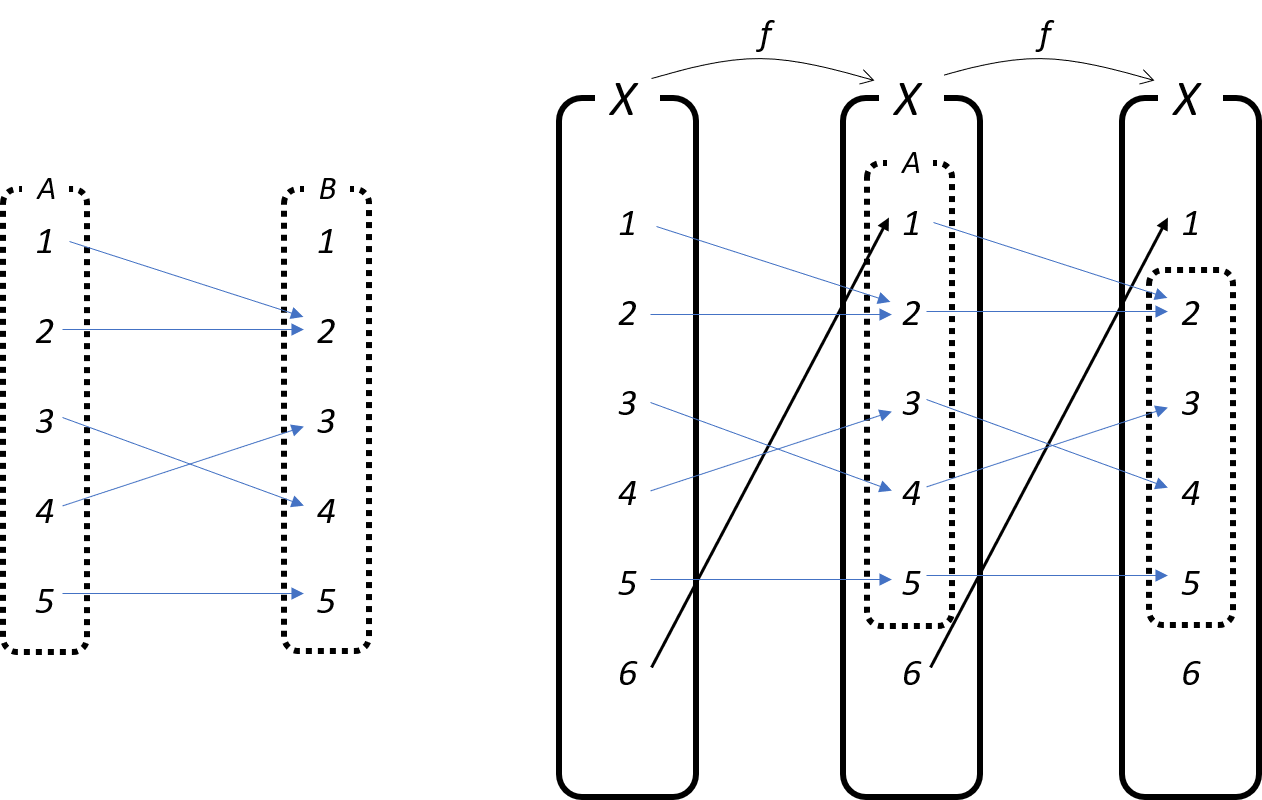
\includegraphics[width=.5\columnwidth]{+17_4}
\caption*{\(f\circ f\text{의 치역}=\{2,3,4,5\}\)}
\end{figure*}
\par
\begin{figure*}[h!]
\centering
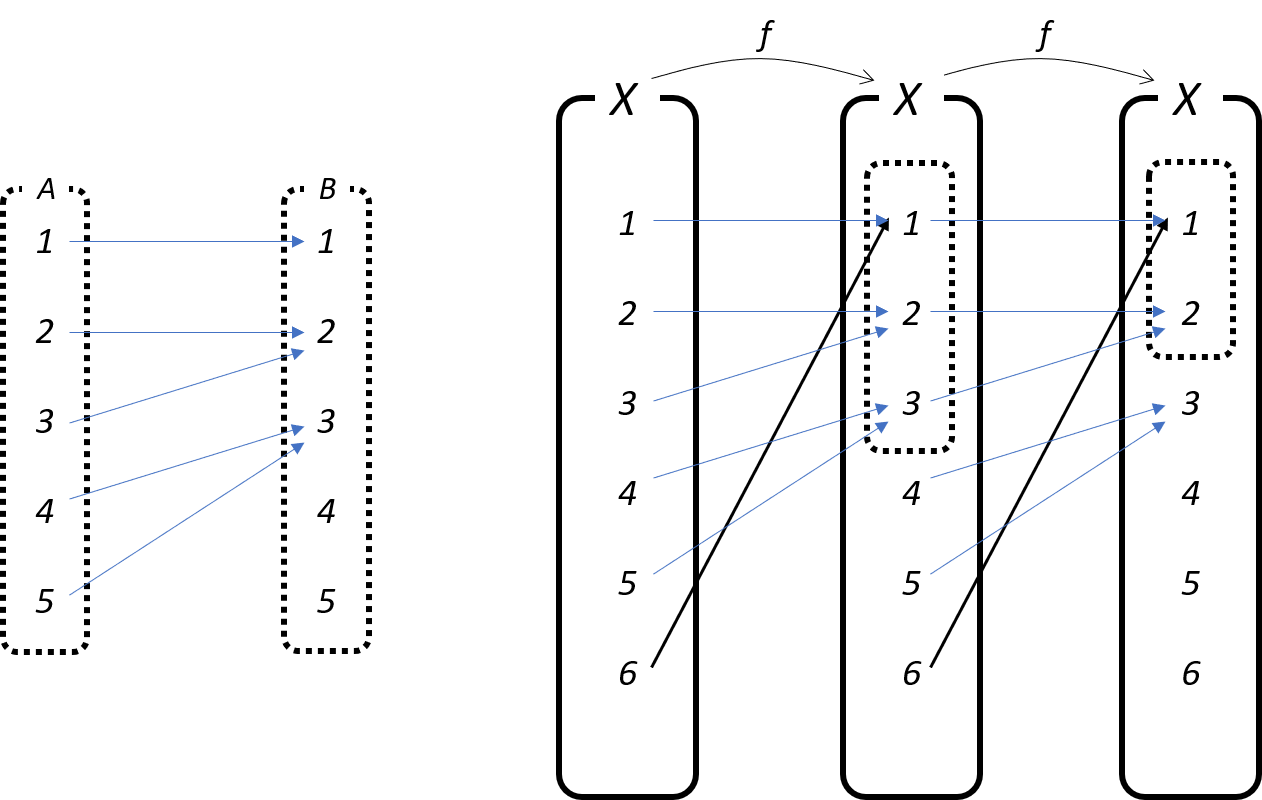
\includegraphics[width=.5\columnwidth]{+17_5}
\caption*{\(f\circ f\text{의 치역}=\{1,2\}\)}
\end{figure*}

\newpage
\begin{multicols*}{2}
%
\prob{나형 14번}
\begin{center}
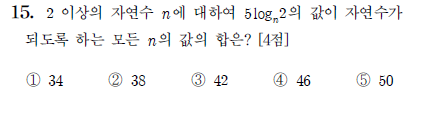
\includegraphics[width=\columnwidth]{-15}
\end{center}
\vfill\null\columnbreak
\(5\log_n2=k\)
라고 두면
\[\log_n2^5=k\]
이므로
\[n^k=2^5\]
이고
\[n=2^{\frac5k}\]
이다
(단, \(n\), \(k\)는 자연수이고 \(n\ge2\)).
\(2^{\frac5k}\)의 값이 자연수이려면 \(k\)는 \pb1이거나 \pb5일 수밖에 없다.
이때 \(n\)의 값은 각각 \(\pb{32}\)이거나 \pb2이다.
\end{multicols*}

\newpage
\begin{multicols*}{2}
%
\prob{나형 20번}
\begin{center}
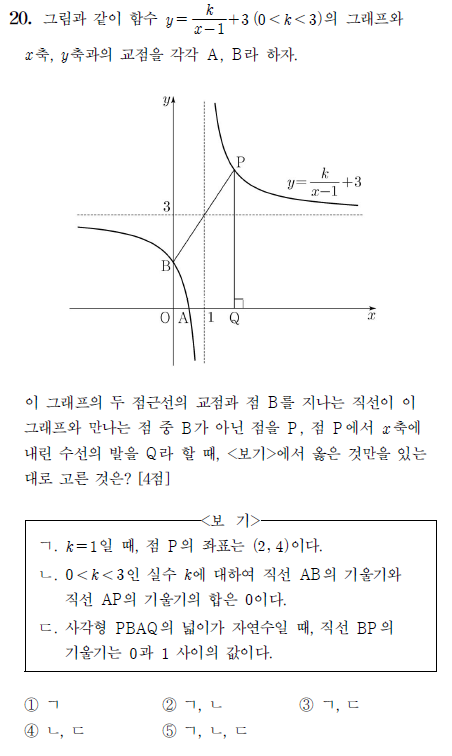
\includegraphics[width=\columnwidth]{-20}
\end{center}
%\vfill\null\columnbreak
ㄱ : 이 유리함수의 그래프는 점 \((1,3)\)에 대하여 대칭이다.
따라서 \(B\)와 \(P\)는 점 \((1,3)\)에 대하여 대칭이다.

\(k=1\)일 때, 이 함수의 그래프에서 \(y\)절편은 \(x=0\)을 대입하여 얻어진다 ;
\[y=\frac1{0-1}+3=2\]
그러므로 \(B=(0,2)\)이다.
\(B(0,2)\)와 \(P(m,n)\)의 중점이 \((1,3)\)이므로
\[\frac{0+m}2=1,\quad\frac{2+n}2=3\]
\(m=2\), \(n=4\)이고 \(P=(2,4)\)이다.

\vfill\null\columnbreak
\noindent
ㄴ : 일반적인 \(k\)에 대하여 각 점들의 좌표를 구해보자.
\(x\)절편을 구하면
\[0=\frac k{x-1}+3\]
\[x=1-\frac k3\]
이므로 \(A=(1-\frac k3,0)\).
\(y\)절편을 구하면
\[y=\frac k{0-1}+3=-k+3\]
이므로 \(B=(0,-k+3)\).
\(P=(m,n)\)으로 두면
\[\frac{0+m}2=1,\quad\frac{-k+3+n}2=3\]
따라서 \(m=\pb{2}\), \(n=\pb{k+3}\)이고 \(P=(\pb2,\pb{k+3})\)이다.

\par\bigskip\noindent
ㄷ. \(\square PBAQ=\square PBOQ-\triangle OAB\)이고 이때 \(\square PBOQ=6\)이고
\begin{align*}
\triangle OAB
&=\frac12\times\left(1-\frac k3\right)\times(-k+3)\\
&=\frac16(-k+3)^2
\end{align*}
이다.
이때 \(\triangle OAB<3\)이므로 \(\triangle OAB=1\)이거나 \(\triangle OAB=2\)이다.
따라서 \(k=\pb{\(3\pm\sqrt6\)}\)이거나 \(k=\pb{\(3\pm2\sqrt3\)}\)이며, \(0<k<3\)임을 고려하면 가능한 \(k\)의 값은 \(k=\pb{\(3-\sqrt6\)}\)이다.
%사각형 \(PBAQ\)보다 넓이가 조금 더 큰 사각형 \(PBOQ\)를 생각하면, 사각형 \(PBOQ\)의 넓이는 \pb6이다.
%이때 \(O\), \(B\), \(A\)로 둘러싸인 부분의 넓이를 \(S\)라고 하면
%\[\square PBAQ=\pb 6-S\]
%이다.
%\(\square PBAQ\)의 넓이가 자연수이려면 \(S\) 또한 자연수여야 한다.
%%가능한 \(S\)의 값은 \(S=\pb1\)이다.
%이때 \(S<\pb3\)이므로 가능한 \(S\)의 값은 \pb1과 \pb2이다.
\end{multicols*}

\newpage
\begin{multicols*}{2}
%
\prob{나형 26번}
\begin{center}
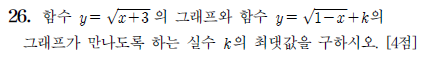
\includegraphics[width=\columnwidth]{-26}
\end{center}
\vfill\null\columnbreak

\(y=\sqrt{x+3}\)의 그래프는 꼭짓점이 \((-3,0)\)이고 오른쪽 위로 뻗는 그래프이다.
\(y=\sqrt{1-x}+k\)의 그래프는 꼭짓점이 \((1,k)\)이고 왼쪽 위로 뻗는 그래프이다.
\(k\)의 값을 변화해가며 생각해보면 \(k\le\pb2\)이다.
\begin{center}
\centering
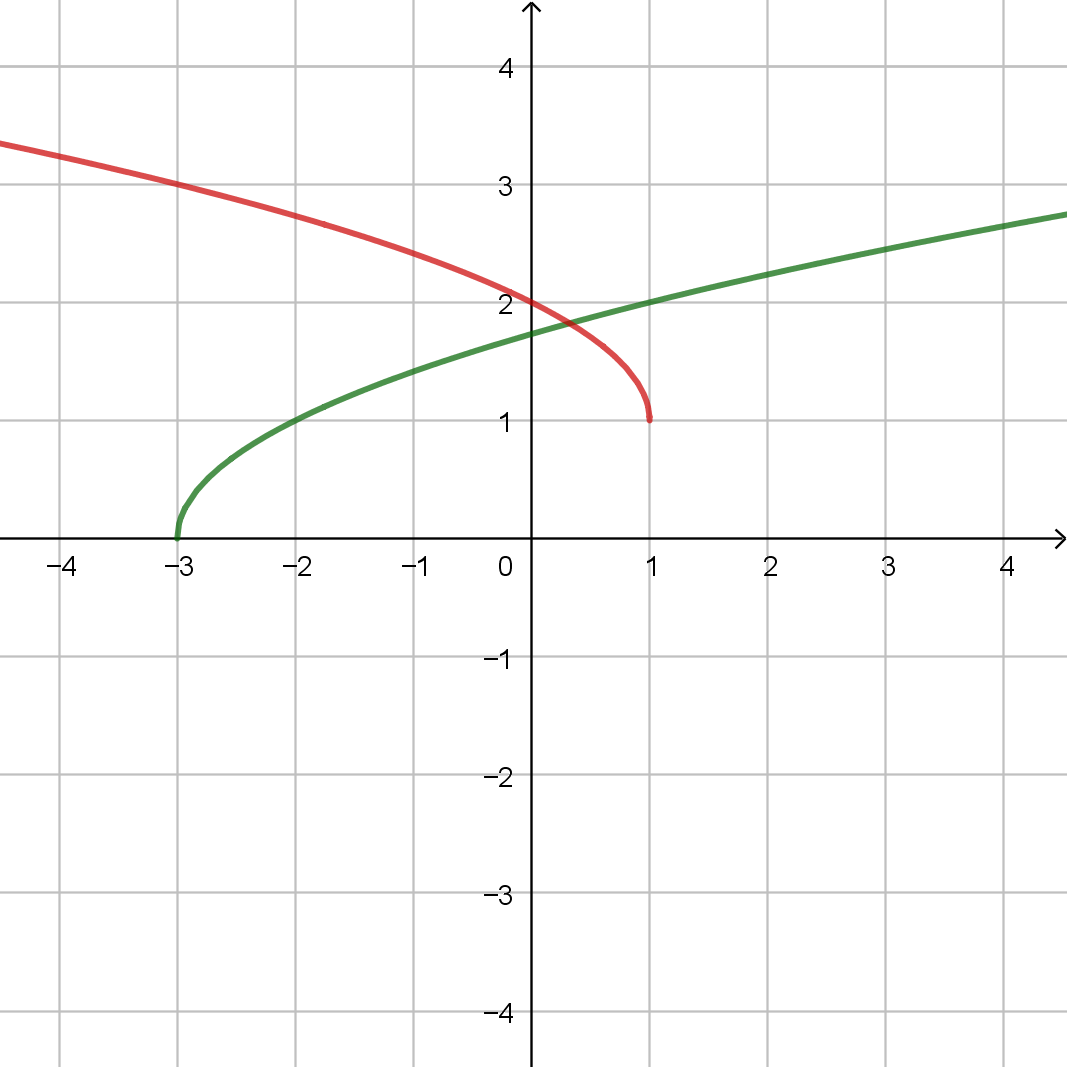
\includegraphics[width=.8\columnwidth]{-26_1}
\par\(k=1\)\par\bigskip\bigskip
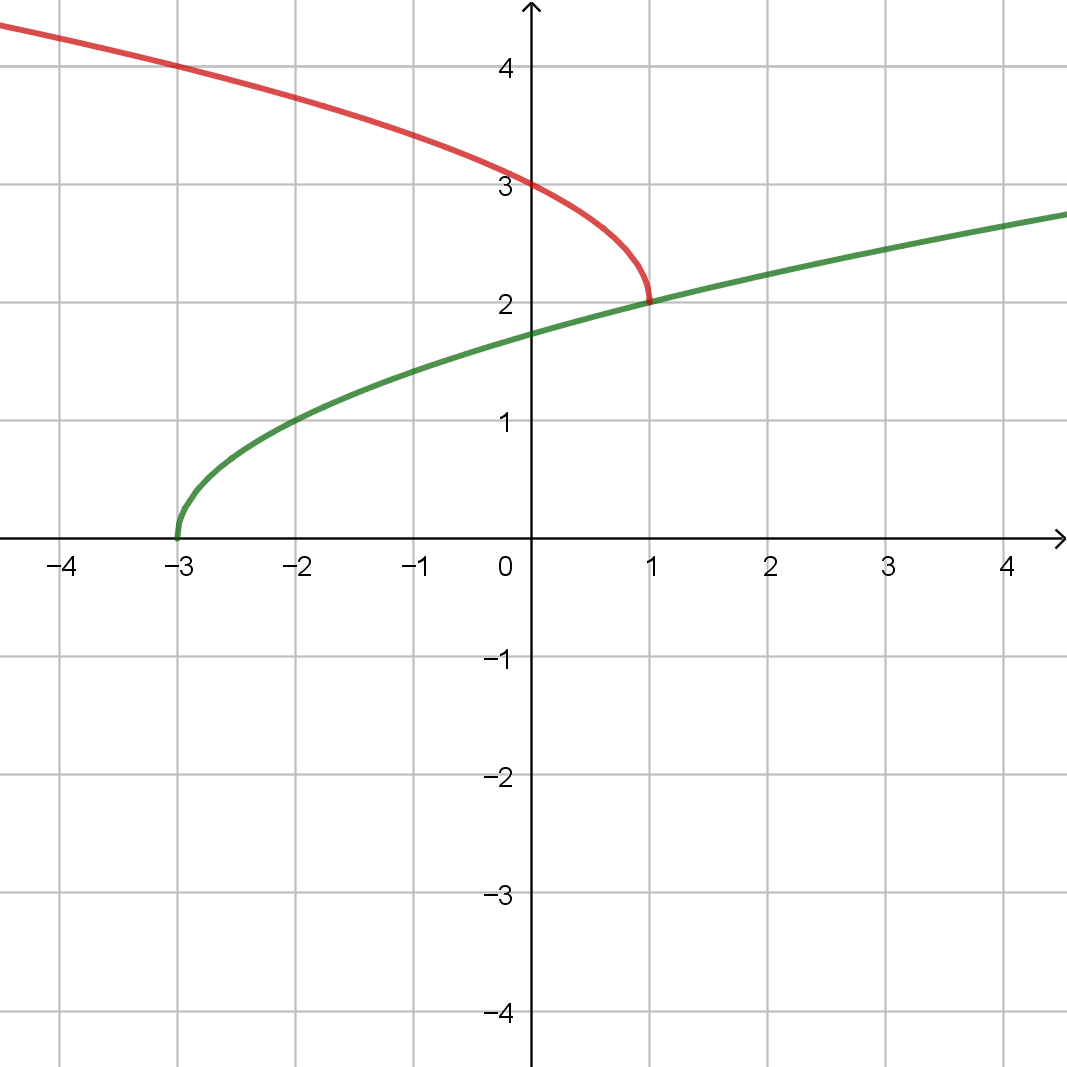
\includegraphics[width=.8\columnwidth]{-26_2}
\par\(k=2\)\par\bigskip\bigskip
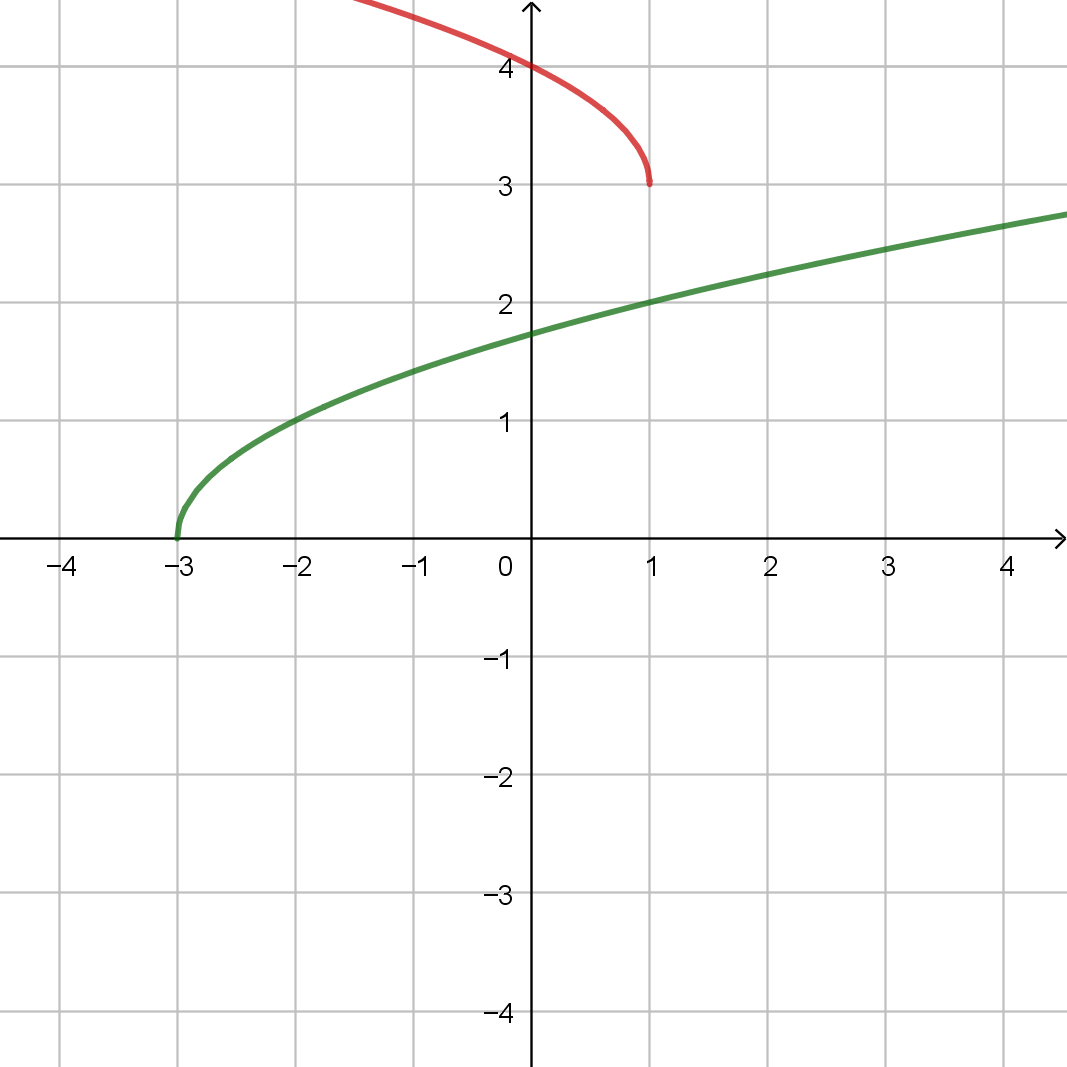
\includegraphics[width=.8\columnwidth]{-26_3}
\par\(k=3\)\par\bigskip\bigskip
\end{center}

\end{multicols*}

\end{document}